\chapter{Ciclo di isteresi}

\renewcommand\thesection{\Roman{section}}

\textbf{Obiettivo:} Determinare i rapporti di trasformazione, visualizzare il ciclo di isteresi dei lamierini magnetici componenti un trasformatore e determinare la resistenza interna di un oscilloscopio.

\paragraph{Strumentazione:} 
\begin{enumerate}
    \item il circuito pre-costruito con i trasformatori;
    \item una resistenza di circa $\SI{500}{\kilo\Omega}$ e un condensatore di capacità tale che $RC\gg T=\SI{20}{ms}$;
    \item un oscilloscopio.
\end{enumerate}

\paragraph{Procedura:}
\begin{enumerate}
    \item usando i due canali dell'oscilloscopio misurare le tensioni delle boccole A e B riferite a G (ground) che rappresenta la massa del sistema;
    \begin{figure}[h]
        \centering
        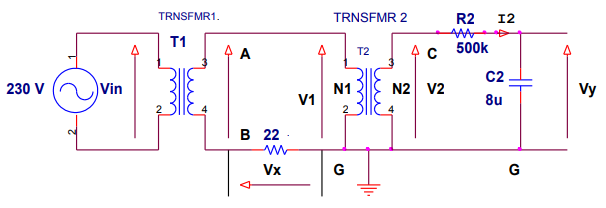
\includegraphics[width=0.8\linewidth]{Immagini/EXP2 - circuito ciclo isteresi.png}
        \caption{circuito per visualizzare il ciclo di isteresi.}
        \label{fig: EXP2 - circuito ciclo isteresi}
    \end{figure}
    \item ricavare la tensione $V_{AB}\sin{\omega t}$ in uscita dal primo trasformatore con le funzioni MATH dell'oscilloscopio, la tensione $V_{AB}$ è il valore massimo;
    \item ricavare il rapporto di trasformazione del primario e del secondario sapendo che
    \begin{equation}
        n_1=\frac{N_{p}}{N_{s}}=\frac{230}{V_{AB,eff}};
    \end{equation}
    \item misurare la tensione $V_{CG}$ e calcolare il rapporto di trasformazione del secondo trasformatore con 
    \begin{equation}
        n_2=\frac{N_p'}{N_s'}=\frac{V_{BG}}{V_{CD}};
    \end{equation}
    \item inserire fra C e D la resistenza, inserire tra D e G il condensatore e misurare la tensione $V_{DG}$;
    \item impostare l'oscilloscopio in funzionamento X-Y ed applicare al canale X la $V_{BG}$ ed al canale Y la $V_{DG}$: si vedrà sullo schermo il ciclo di isteresi;
    \item sostituire il condensatore con l'oscilloscopio e misurare le tensioni $V_{CG}$ e $V_{DG}$;
    \item risolvere per $R_i$ la relazione
    \begin{equation}
        \frac{V_{CG}R_i}{R+R_i}=V_{DG}.
    \end{equation}
\end{enumerate}

\setcounter{section}{0}
\renewcommand\thesection{\Alph{section}}

\section{Visualizzazione del ciclo d'isteresi}
Per visualizzare il ciclo di isteresi di lamierini magnetici componenti un trasformatore, si può usare il circuito in figura \ref{fig: EXP2 - circuito ciclo isteresi}. Scrivendo l'equazione di maglia del primario si ha
\begin{equation}
    v_1 - L_1 \frac{d i_1}{dt} - M\frac{d i_2}{dt} = R_1i_1.
\end{equation}
Ricordando che $Hl=N_1i_1+N_2i_2$, dove $l$ è la lunghezza del circuito magnetico, si ha che $H\propto N_1i_1\propto i_1R_1 \propto v_{R_1}=v_X$. Nel circuito del secondario si ha
\begin{equation}
    v_2 = N_2 \frac{d\Phi}{dt} = N_2S\frac{dB}{dt}m\quad\therefore\quad dB=\frac{v_2}{N_2S}dt,
    \label{placeholder_label}
\end{equation}
la quale integrata restituisce
\begin{equation}
    B=\frac{1}{N_2S}\int v_2dt+C=\frac{1}{N_2S}v_y+C.
\end{equation}
Inviando sul canale X dell'oscilloscopio la tensione $v_x$ e sul canale Y la tensione $v_y$ si ottiene disegnato sullo schermo il ciclo di isteresi.